% presentation
\documentclass{beamer}
\usetheme[height=7mm]{Rochester}
\usecolortheme{rose}

% handout

%\documentclass[handout]{beamer}
%\usepackage{pgfpages} \pgfpagesuselayout{8 on 1}[a4paper]

%\documentclass[mathserif]{article}
%\usepackage{beamerarticle}

\usepackage{amsmath}
\usepackage{comment}
\usepackage{amssymb,amsfonts}
\usepackage[T1]{fontenc}
\usepackage{lmodern}
\usepackage{tikz}
\usepackage{simpsons}
\usepackage{marvosym}
\usepackage{color}
\usepackage{multirow}
\usepackage{pgffor}
\usepackage[slide,algoruled,titlenumbered,vlined,noend,linesnumbered,]{algorithm2e}

\usefonttheme{structurebold}

\setbeamertemplate{footline}[frame number]
\setbeamertemplate{navigation symbols}{}
\setbeamerfont{smallverb}{size*={73}}
\usefonttheme[onlymath]{serif}
\setbeamertemplate{theorems}[numbered]
\newtheorem{construction}[theorem]{Construction}
\newtheorem{proposition}[theorem]{Proposition}

\AtBeginSection[] { 
  \begin{frame} 
    \frametitle{Content} 
    \tableofcontents[currentsection]
  \end{frame} 
  \addtocounter{framenumber}{-1} 
}

\usetikzlibrary[shapes.arrows]
\usetikzlibrary{shapes.geometric}
\usetikzlibrary{backgrounds}
\usetikzlibrary{positioning}
\usetikzlibrary{calc}
\usetikzlibrary{intersections}
\usetikzlibrary{fadings}
\usetikzlibrary{decorations.footprints}
\usetikzlibrary{patterns}
\usetikzlibrary{shapes.callouts}
\usetikzlibrary{fit}
%handout

\providecommand{\abs}[1]{\lvert#1\rvert}

\tikzset{every picture/.style={line width=1pt,show background rectangle},background rectangle/.style={fill=blue!10,rounded corners=2ex}}

\author{Yu Zhang}
\institute{Harbin Institute of Technology}
\date[Crypt'16A]{Cryptography, Autumn, 2016}

%% presentation
\documentclass{beamer}
\usetheme[height=7mm]{Rochester}
\usecolortheme{rose}

% handout

%\documentclass[handout]{beamer}
%\usepackage{pgfpages} \pgfpagesuselayout{8 on 1}[a4paper]

%\documentclass[mathserif]{article}
%\usepackage{beamerarticle}

\usepackage{amsmath}
\usepackage{comment}
\usepackage{amssymb,amsfonts}
\usepackage[T1]{fontenc}
\usepackage{lmodern}
\usepackage{tikz}
\usepackage{simpsons}
\usepackage{marvosym}
\usepackage{color}
\usepackage{multirow}
\usepackage{pgffor}
\usepackage[slide,algoruled,titlenumbered,vlined,noend,linesnumbered,]{algorithm2e}

\usefonttheme{structurebold}

\setbeamertemplate{footline}[frame number]
\setbeamertemplate{navigation symbols}{}
\setbeamerfont{smallverb}{size*={73}}
\usefonttheme[onlymath]{serif}
\setbeamertemplate{theorems}[numbered]
\newtheorem{construction}[theorem]{Construction}
\newtheorem{proposition}[theorem]{Proposition}

\AtBeginSection[] { 
  \begin{frame} 
    \frametitle{Content} 
    \tableofcontents[currentsection]
  \end{frame} 
  \addtocounter{framenumber}{-1} 
}

\usetikzlibrary[shapes.arrows]
\usetikzlibrary{shapes.geometric}
\usetikzlibrary{backgrounds}
\usetikzlibrary{positioning}
\usetikzlibrary{calc}
\usetikzlibrary{intersections}
\usetikzlibrary{fadings}
\usetikzlibrary{decorations.footprints}
\usetikzlibrary{patterns}
\usetikzlibrary{shapes.callouts}
\usetikzlibrary{fit}
%handout

\providecommand{\abs}[1]{\lvert#1\rvert}

\tikzset{every picture/.style={line width=1pt,show background rectangle},background rectangle/.style={fill=blue!10,rounded corners=2ex}}

\author{Yu Zhang}
\institute{Harbin Institute of Technology}
\date[Crypt'16A]{Cryptography, Autumn, 2016}

%\input{1introduction.tex}
%\input{2perfectlysecret.tex}
%\input{3privatekey.tex}


\title{Introduction}

\begin{document}
\maketitle
\begin{frame}
\frametitle{Outline}
\tableofcontents
\end{frame}
\section{Cryptography and Modern Cryptography}
\begin{frame}\frametitle{What is Cryptography?}
\begin{itemize}
\item \textbf{Cryptography}: from Greek \emph{krypt\'os}, ``hidden, secret''; and \emph{gr\'{a}phin}, ``writing''.
\item \textbf{Cryptography}: the art of writing or solving codes.\\ (Concise oxford dictionary 2006)
\item \textbf{Codes}: a system of prearranged signals, especially used to ensure secrecy in transmitting messages. \\ (\emph{code word} in cryptography)
\item \textbf{1980s}: from Classic to Modern; from Military to Everyone.
\item \textbf{Modern cryptography}: the scientific study of techniques for securing digital information, transactions, and distributed computations.
\end{itemize}
\end{frame}
\section{The Setting of Private-Key Encryption}
\begin{frame}\frametitle{Private-Key Encryption}
\begin{itemize}
\item \textbf{Goal}: to construct a \textbf{ciphers} (encryption schemes) for providing secret communication between two parties sharing \textbf{private-key} (the symmetric-key) in advance.
\item \textbf{Implicit assumption}: there is some way of initially sharing a key in a secret manner.
\item \textbf{Disk encryption}: the same user at different points in time.
\end{itemize}
\end{frame}
\begin{frame}\frametitle{The Syntax of Encryption}
\begin{figure}
\begin{center}
\begin{tikzpicture}
\node (sender) {\Lisa};
\node (bart) [below of = sender] {Alice};
\node (enc) [draw, right of = sender, rounded corners=1ex,node distance = 2cm] {$\mathsf{Enc}$};
\node (k1) [above of = enc, node distance = 1cm] {$k$};
\node (c) [right of = enc, node distance = 2cm] {$c$};
\node (gen) [draw, above of = c, rounded corners=1ex,node distance = 1cm] {$\mathsf{Gen}$};
\node (adv) [below of = c, node distance = 1cm] {\Burns};
\node (burns) [below of = adv] {Adversary};
\node (dec) [draw, right of = c, rounded corners=1ex,node distance = 2cm] {$\mathsf{Dec}$};
\node (k2) [above of = dec, node distance = 1cm] {$k$};
\node (receiver) [right of = dec, node distance = 2cm] {\Left\Bart};
\node (lisa) [below of = receiver] {Bob};
\draw[-latex] (sender) -- (enc) node [midway, above] {$m$};
\draw (enc) -- (c); \draw[-latex] (c) -- (dec);
\draw[-latex] (dec) -- (receiver) node [midway, above] {$m$};
\draw[-latex] (k1) -- (enc);
\draw[-latex] (gen) -- (k1);
\draw[-latex] (gen) -- (k2);								
\draw[-latex] (k2) -- (dec);		
\end{tikzpicture}
\end{center}
\end{figure}
\begin{itemize}
\item key $k \in \mathcal{K}$, plaintext (or message) $m \in \mathcal{M}$, ciphertext $c \in \mathcal{C}$.
\item \textbf{Key-generation} algorithm~$k \gets \mathsf{Gen}$.
\item \textbf{Encryption} algorithm~$c:= \mathsf{Enc}_k(m)$.
\item \textbf{Decryption} algorithm~$m:= \mathsf{Dec}_k(c)$.
\item \textbf{Encryption scheme}: $\Pi = (\mathsf{Gen}, \mathsf{Enc}, \mathsf{Dec})$.
\item \textbf{Basic correctness requirement}: $\mathsf{Dec}_k(\mathsf{Enc}_k(m)) = m$.
\end{itemize}
\end{frame}
\begin{frame}\frametitle{Securing Key vs Obscuring Algorithm}
\begin{itemize}
\item Easier to maintain secrecy of a short key.
\item In case the key is exposed, easier for the honest parties to change the key.
\item In case many pairs of people, easier to use the same algorithm, but different keys.
\end{itemize}
\begin{alertblock}{Kerckhoffs's principle}
\begin{quote}
The cipher method must not be required to be secret, and it must be able to fall into the hands of the enemy without inconvenience.
\end{quote}	
\end{alertblock}
\end{frame}
\begin{frame}\frametitle{Why ``Open Cryptographic Design''}
\begin{itemize}
\item Published designs undergo public scrutiny are to be stronger.
\item Better for security flaws to be revealed by ``ethical hackers''.
\item Reverse engineering of the code (or leakage by industrial espionage) poses a serious threat to security.
\item Enable the establishment of standards.
\end{itemize}
\end{frame}
\begin{frame}\frametitle{Attack Scenarios}	
\begin{itemize}
\item \textbf{Ciphertext-only}: the adversary just observes ciphertext
\item \textbf{Known-plaintext}: the adversary learns pairs of plaintexts/ciphertexts under the same key
\item \textbf{Chosen-plaintext}: the adversary has the ability to obtain the encryption of plaintexts of its choice
\item \textbf{Chosen-ciphertext}: the adversary has the ability to obtain the decryption of \textbf{other} ciphertexts of its choice
\item \textbf{Passive attack}: COA KPA
\begin{itemize}
\item because not all ciphertext are confidential
\end{itemize}
\item \textbf{Active attack}: CPA CCA
\begin{itemize}
\item when to encrypt/decrypt whatever an adversary wishes?
\end{itemize}
\end{itemize}	
\end{frame}
\section{Historical Ciphers and Their Cryptanalysis}
\begin{comment}
	\begin{frame}\frametitle{Why We Learn Broken Ciphers?}
	\begin{itemize}
	\item To understand the weaknesses of an ``ad-hoc'' approach
	\item To learn that ``simple'' approaches are unlikely to succeed
	\item To feel that ``we are smart enough to do some crypt-analyzing''
	\end{itemize}
	\end{frame}
\end{comment}

\begin{frame}[fragile]\frametitle{Caesar's Cipher}
\begin{quote}
If he had anything confidential to say, he wrote it in cipher, that is, by so changing the order of the letters of the alphabet, that not a word could be made out. If anyone wishes to \alert{decipher} these, and get at their meaning, he must \alert{substitute the fourth letter of the alphabet, namely D, for A}, and so with the others

\rightline{--Suetonius,``Life of Julius Caesar''}
\end{quote}
\begin{itemize}
	\item $\mathsf{Enc}(m)=m+3\mod 26$ \footnote{In fact the quote indicates that decryption involved rotating letters of the alphabet forward 3 positions, $\mathsf{Dec}(c)=c+3\mod 26$}
	\item \textbf{Weakness}: \alert{What is the key?}
\end{itemize}
\begin{exampleblock}{Example}
\verb|begintheattacknow|
%\verb|EHJLQWKHDWWDFNQRZ|
\end{exampleblock}
\end{frame}
\begin{frame}[fragile]\frametitle{Shift Cipher}
\begin{itemize}
\item $\mathsf{Enc}_k(m)=m+k\mod 26$
\item $\mathsf{Dec}_k(c)=c-k\mod 26$
\item \textbf{Weakness}: Fragile under \textbf{Brute-force attack} (exhaustive search)
\end{itemize}
\begin{exampleblock}{Example: Decipher the string}	
\verb|EHJLQWKHDWWDFNQRZ|
\end{exampleblock}
\begin{alertblock}{Sufficient Key Space Principle}
Any secure encryption scheme must have a key space that is not vulnerable to exhaustive search.\footnote{If the plaintext space is larger than the key space.}
\end{alertblock}
\end{frame}
\begin{frame}\frametitle{Index of Coincidence (IC) Method (to find $k$)}
\textbf{Index of Coincidence (IC)}: the probability that two randomly selected letters (pick-then-return) will be identical.

Let $p_i$ denote the probability of $i$th letter in English text.
\[I \overset{\text{def}}{=}\sum_{i=0}^{25} p_i^2 \]
\begin{exampleblock}{Example}
What's the IC of `apple'?
\end{exampleblock}

For a long English text, the IC is $\approx 0.065$.
For $j = 0, 1, \dotsc , 25$, $q_j$ is the probability of $j$th letter in the ciphertext.
\[I_j \overset{\text{def}}{=}\sum_{i=0}^{25} p_i \cdot q_{i+j}\]
\alert{Q: For shift cipher, if $j = k$, then $I_j \approx$ ?}

\end{frame}
\begin{frame}[fragile]\frametitle{Mono-Alphabetic Substitution}
\begin{itemize}
\item \textbf{Idea}: To map each character to a different one in an arbitrary manner.
\item \textbf{Strength}: Key space is large $\approx 2^{88}$. \alert{Q: how to count?}
\item \textbf{Weakness}: The mapping of each letter is fixed.
\end{itemize}
\begin{exampleblock}{Example}
\verb|abcdefghijklmnopqrstuvwxyz|\\
\verb|XEUADNBKVMROCQFSYHWGLZIJPT|

Plaintext: \verb|tellhimaboutme|\\
Ciphertext: \verb|??????????????|
\end{exampleblock}
\end{frame}
\begin{frame}[fragile]\frametitle{Attack with Statistical Patterns}
\begin{enumerate}
\item Tabulate the frequency of letters in the ciphertext.
\item Compare it to those in English text.
\item Guess the most frequent letter corresponds to \verb|e|, and so on.
\item Choose the plaintext that does ``make sense''. (Not trivial)
\end{enumerate}
\begin{table}
\begin{center}
\caption{Average letter frequencies for English-language text}
\begin{tabular}{|cc|cc|cc|cc|cc|} \hline
e & 12.7\% & t & 9.1\% & a & 8.2\% & o & 7.5\% & i & 7.0\%\\
n & 6.7\% & \_ & 6.4\% & s & 6.3\% & h & 6.1\% & r & 6.0\%\\
d & 4.3\% & l & 4.0\% & c & 2.8\% & u & 2.8\% & m & 2.4\%\\
w & 2.4\% & f & 2.2\% & g & 2.0\% & y & 2.0\% & p & 1.9\%\\
b & 1.5\% & v & 1.0\% & k & 0.8\% & j & 0.2\% & x & 0.2\%\\
q & 0.1\% & z & 0.1\% & & & & & &\\ \hline
\end{tabular}
\end{center}
\end{table}
\end{frame}
\begin{frame}[fragile]\frametitle{Example of Frequency Analysis (Ciphertext)}
\begin{verbatim}
LIVITCSWPIYVEWHEVSRIQMXLEYVEOIEWHRXEXIPFEMVEWHKVS
TYLXZIXLIKIIXPIJVSZEYPERRGERIMWQLMGLMXQERIWGPSRIH
MXQEREKIETXMJTPRGEVEKEITREWHEXXLEXXMZITWAWSQWXSWE
XTVEPMRXRSJGSTVRIEYVIEXCVMUIMWERGMIWXMJMGCSMWXSJO
MIQXLIVIQIVIXQSVSTWHKPEGARCSXRWIEVSWIIBXVIZMXFSJX
LIKEGAEWHEPSWYSWIWIEVXLISXLIVXLIRGEPIRQIVIIBGIIHM
WYPFLEVHEWHYPSRRFQMXLEPPXLIECCIEVEWGISJKTVWMRLIHY
SPHXLIQIMYLXSJXLIMWRIGXQEROIVFVIZEVAEKPIEWHXEAMWY
EPPXLMWYRMWXSGSWRMHIVEXMSWMGSTPHLEVHPFKPEZINTCMXI
VJSVLMRSCMWMSWVIRCIGXMWYMX
\end{verbatim}
\end{frame}
\begin{frame}[fragile]\frametitle{Example of Frequency Analysis (Analysis)}
Count and Guess, Trial and Error.
\begin{table}
\begin{center}
\caption{Analysis Steps}
\begin{tabular}{|r|l|} \hline
Ciphertext & Plaintext \\ \hline
\alert{I}   & \alert{e} \\
\alert{XLI} & \alert{the} \\
\alert{E} & \alert{a} \\
\alert{R}tate & \alert{s}tate \\
atthatt\alert{MZ}e & atthatt\alert{im}e \\
he\alert{V}e & he\alert{r}e \\
remar\alert{A} & remar\alert{k} \\ \hline
\end{tabular}
\end{center}
\end{table}
\end{frame}
\begin{frame}[fragile]\frametitle{Example of Frequency Analysis (Plaintext)}
\begin{quote}
Hereupon Legrand arose, with a grave and stately air, and brought me the beetle
from a glass case in which it was enclosed. It was a beautiful scarabaeus, and, at
that time, unknown to naturalists -- of course a great prize in a scientific point
of view. There were two round black spots near one extremity of the back, and a
long one near the other. The scales were exceedingly hard and glossy, with all the
appearance of burnished gold. The weight of the insect was very remarkable, and,
taking all things into consideration, I could hardly blame Jupiter for his opinion
respecting it.

\rightline{--Edgar Allan Poe's ``The Gold-Bug''}
\end{quote}
\end{frame}

\begin{frame}[fragile]\frametitle{Vigen\`{e}re (poly-alphabetic shift) Cipher}
\begin{itemize}
\item \textbf{Idea}: To ``smooth out'' the distribution in the ciphertext by mapping different instances of the same letter in the plaintext to different ones in the ciphertext
\item \textbf{Encryption}: $c_i=m_i+k_{[i\bmod t]}$, $t$ is the length (period) of $k$
\item \textbf{Cryptanalysis}: Need find $t$; if $t$ is known, need know whether the decryption ``makes sense'', but brute force ($26^t$) is infeasible for $t > 15$
\end{itemize}
\begin{exampleblock}{Example (Key is `cafe')}
\begin{description}[Ciphertext]
\item[Plaintext]  \verb|tellhimaboutme| \\
\item[Key]        \verb|cafecafecafeca| \\
\item[Ciphertext] \verb|??????????????| %\verb|WFRQKJSFEPAYPF|
\end{description}
\end{exampleblock}
\end{frame}
\begin{frame}[fragile]\frametitle{Kasiski's Method (to find $t$)}
\begin{itemize}
\item To identify repeated patterns of length 2 or 3.
\item The distance between such appearances is a multiple of $t$.
\item $t$ is the greatest common divisor of all the distances.
\end{itemize}
\begin{exampleblock}{Example (Key is `beads')}
\begin{semiverbatim}
themanandthewomanretrievedtheletterfromthepostoffice
beadsbeadsbeadsbeadsbeadsbeansdeadsbeadsbeadsbeadbea
VMFQTPFOH\alert{MJJ}XSFCSSIMTNFZXFYISEIYUIKHWPQ\alert{MJJ}QSLVTGJKGF
\end{semiverbatim}
\end{exampleblock}
\end{frame}
\begin{frame}\frametitle{Index of Coincidence (IC) Method (to find $t$)}
For $\tau = 1, 2, \dotsc$, $q_i$ is the probability of $i$th letter in $c_1, c_{1+\tau}, c_{1+2\tau}, \dotsc$, IC is
\[I_\tau \overset{\text{def}}{=}\sum_{i=0}^{25} q_i^2\]
\alert{If $\tau = t$, then $I_\tau \approx ?$} ; otherwise $q_i \approx \frac{1}{26}$ and
\[I_\tau \approx \sum_{i=0}^{25} \left(\frac{1}{26}\right)^2 \approx 0.038\]
Then reuse IC method to find $k_i$.
\begin{alertblock}{Arbitrary Adversary Principle}
Security must be guaranteed for any adversary within the class of adversaries having the specified power
\end{alertblock}
\end{frame}
\begin{frame}\frametitle{Cryptanalytic Attacks (homework assignment)}
\begin{itemize}
\item Under COA, the requirement for ciphertext related to the size of the key space.  Vig\`{e}nere > mono-alphabetic sub. > shift
\item Under KPA, trivially broken.
\end{itemize}
\begin{alertblock}{Lessons learned}
\begin{itemize}
\item Sufficient key space principle.
\item Designing secure cipher is a hard task.
\item Complexity does not imply security. (then what does?)
\item Arbitrary adversary principle
\end{itemize}
\end{alertblock}
\end{frame}
\section{The Basic Principles of Modern Cryptography}
\begin{frame}\frametitle{Three Main Principles of Modern Cryptography}
\begin{enumerate}
\item The formulation of a rigorous \textbf{definition} of security / threat model.
\item When the security of a cipher relies on an unproven \textbf{assumption}, this assumption must be precisely stated and be as minimal as possible.
\item Cipher should be accompanied by a rigorous \textbf{proof} of security with the above definition and the above assumption.
\end{enumerate}
\end{frame}
\begin{frame}\frametitle{Why Principle 1 -- Formulation of Exact Definitions}
\begin{exampleblock}{Q: how would you formalize the security for private-key encryption?}
\begin{enumerate}
\item \emph{No adversary can find the secret key when given a ciphertext.}\\
$\mathsf{Enc}_k(m)=m$
\item \emph{No adversary can find the plaintext that corresponds to the ciphertext.}\\
$\mathsf{Enc}_k(m)=m_{0}\| \mathsf{AES}_k(m)$
\item \emph{No adversary can determine any character of the plaintext that corresponds to the ciphertext.}\\
$m=1000$, someone can learn $ 800 < m < 1200$
\item \emph{No adversary can derive any meaningful information about the plaintext from the ciphertext.}\\
Could you define so-called `meaningful'?
\end{enumerate}
\emph{\alert{Definitions of security should suffice for all potential applications.}}
\end{exampleblock}
\end{frame}
\begin{frame}\frametitle{Why Principle 1 -- How to define}
%\begin{exampleblock}{General Form}
%A cryptographic scheme for a given \textbf{task} is secure if no adversary of a specified \textbf{power} can achieve a specified \textbf{break}
%\end{exampleblock}

How To Define Security -- Lesson From Alan Turing
\begin{itemize}
\item What's computation?\footnote{Q: Any ``mathematical proof that there exist well-defined problems that computers cannot solve''? A: Halting Problem in computability theory}
\begin{enumerate}
\item A direct appeal to \textbf{intuition}
\item A \textbf{proof of the equivalence} of two definitions\\ (The new one has a greater intuitive appeal)
\item Giving \textbf{examples} solved using a definition
\end{enumerate}
\item Additional method for security: \textbf{Test of time}
\end{itemize}
\end{frame}	
\begin{frame}\frametitle{Principle 2 -- Reliance on Precise Assumptions}
Most cryptographic constructions \textbf{cannot be proven secure unconditionally}
\begin{itemize}
	\item \textbf{Why?} 
	\begin{enumerate}
		\item Validation of the assumption
		\item Comparison of schemes
		\item Facilitation of proofs of security
	\end{enumerate}
	\textbf{The construction is secure if the assumption is true.}
	\item \textbf{How?} 
	\begin{enumerate}
		\item old, so well tested
		\item simple and lower-level, so easy to study, refute \& correct
	\end{enumerate}
\end{itemize}
\end{frame}
\begin{frame}\frametitle{Principle 3 -- Rigorous Proofs of Security}
\begin{itemize}
\item \textbf{Why?} Proofs are more desirable in computer security than in other fields.
\item \textbf{The reductionist approach}: 
\begin{theorem}	Given that Assumption X is true, Construction Y is secure according to the given definition.
\end{theorem}
\begin{proof} Reduce the problem given by X to the problem of breaking Y.
\end{proof}
\item \textbf{Ad-hoc approaches}: for those who need a ``quick and dirty'' solution, or who are just simply unaware.
\end{itemize}
\end{frame}
\begin{frame}\frametitle{Summary}
\begin{itemize}
\item Cryptography secures information, transactions and computations
\item Kerckhoffs's principle \& Open cryptographic design
\item Caesar's, shift, Mono-Alphabetic sub., Vigen\`{e}re
\item Brute force, letter frequency, Kasiski's, IC
\item Sufficient key space principle
\item Arbitrary adversary principle
\item Rigorously proven security
\end{itemize}
\end{frame}
\end{document}


%% presentation
\documentclass{beamer}
\usetheme[height=7mm]{Rochester}
\usecolortheme{rose}

% handout

%\documentclass[handout]{beamer}
%\usepackage{pgfpages} \pgfpagesuselayout{8 on 1}[a4paper]

%\documentclass[mathserif]{article}
%\usepackage{beamerarticle}

\usepackage{amsmath}
\usepackage{comment}
\usepackage{amssymb,amsfonts}
\usepackage[T1]{fontenc}
\usepackage{lmodern}
\usepackage{tikz}
\usepackage{simpsons}
\usepackage{marvosym}
\usepackage{color}
\usepackage{multirow}
\usepackage{pgffor}
\usepackage[slide,algoruled,titlenumbered,vlined,noend,linesnumbered,]{algorithm2e}

\usefonttheme{structurebold}

\setbeamertemplate{footline}[frame number]
\setbeamertemplate{navigation symbols}{}
\setbeamerfont{smallverb}{size*={73}}
\usefonttheme[onlymath]{serif}
\setbeamertemplate{theorems}[numbered]
\newtheorem{construction}[theorem]{Construction}
\newtheorem{proposition}[theorem]{Proposition}

\AtBeginSection[] { 
  \begin{frame} 
    \frametitle{Content} 
    \tableofcontents[currentsection]
  \end{frame} 
  \addtocounter{framenumber}{-1} 
}

\usetikzlibrary[shapes.arrows]
\usetikzlibrary{shapes.geometric}
\usetikzlibrary{backgrounds}
\usetikzlibrary{positioning}
\usetikzlibrary{calc}
\usetikzlibrary{intersections}
\usetikzlibrary{fadings}
\usetikzlibrary{decorations.footprints}
\usetikzlibrary{patterns}
\usetikzlibrary{shapes.callouts}
\usetikzlibrary{fit}
%handout

\providecommand{\abs}[1]{\lvert#1\rvert}

\tikzset{every picture/.style={line width=1pt,show background rectangle},background rectangle/.style={fill=blue!10,rounded corners=2ex}}

\author{Yu Zhang}
\institute{Harbin Institute of Technology}
\date[Crypt'16A]{Cryptography, Autumn, 2016}

%\input{1introduction.tex}
%\input{2perfectlysecret.tex}
%\input{3privatekey.tex}


\title{Perfectly Secret Encryption}

\begin{document}
\maketitle
\begin{frame}\frametitle{Outline}
\tableofcontents
\end{frame}
\section{Definitions and Basic Properties}
\begin{frame}\frametitle{Recall The Syntax of Encryption}
\begin{figure}
\begin{center}
\begin{tikzpicture}
\node (sender) {\Lisa};
\node (bart) [below of = sender] {Alice};
\node (enc) [draw, right of = sender, rounded corners=1ex,node distance = 2cm] {$\mathsf{Enc}$};
\node (k1) [above of = enc, node distance = 1cm] {$k$};
\node (c) [right of = enc, node distance = 2cm] {$c$};
\node (gen) [draw, above of = c, rounded corners=1ex,node distance = 1cm] {$\mathsf{Gen}$};
\node (adv) [below of = c, node distance = 1cm] {\Burns};
\node (burns) [below of = adv] {Adversary};
\node (dec) [draw, right of = c, rounded corners=1ex,node distance = 2cm] {$\mathsf{Dec}$};
\node (k2) [above of = dec, node distance = 1cm] {$k$};
\node (receiver) [right of = dec, node distance = 2cm] {\Left\Bart};
\node (lisa) [below of = receiver] {Bob};
\draw[-latex] (sender) -- (enc) node [midway, above] {$m$};
\draw (enc) -- (c); \draw[-latex] (c) -- (dec);
\draw[-latex] (dec) -- (receiver) node [midway, above] {$m$};
\draw[-latex] (k1) -- (enc);
\draw[-latex] (gen) -- (k1);
\draw[-latex] (gen) -- (k2);								
\draw[-latex] (k2) -- (dec);		
\end{tikzpicture}
\end{center}
\end{figure}
\begin{itemize}
\item $k \in \mathcal{K}, m \in \mathcal{M}, c \in \mathcal{C}$.
\item $k \gets \mathsf{Gen}, c:= \mathsf{Enc}_k(m), m:= \mathsf{Dec}_k(c)$.
\item \textbf{Encryption scheme}: $\Pi = (\mathsf{Gen}, \mathsf{Enc}, \mathsf{Dec})$.
\item \textbf{Random Variable}: $K, M, C$ for key, plaintext, ciphertext.
\item \textbf{Probability}: $\Pr[K=k], \Pr[M=m], \Pr[C=c].$
\item \alert{What's the basic correctness requirement?}
\end{itemize}
\end{frame}
\begin{frame}\frametitle{Definition of `Perfect Secrecy'}
\textbf{Intuition}: An adversary knows the probability distribution over $\mathcal{M}$. $c$ should have no effect on the knowledge of the adversary; the a \emph{posteriori} likelihood that some $m$ was sent should be no different from the a \emph{priori} probability that $m$ would be sent. 
\begin{definition}
$\Pi$ over $\mathcal{M}$ is \textbf{perfectly secret} if for every probability distribution over $\mathcal{M}$, $\forall m \in \mathcal{M}$ and $\forall c \in \mathcal{C}$ for which $\Pr[C = c] > 0$:
\[ \Pr[M=m | C=c] = \Pr[M=m].\]
\end{definition}
\textbf{Simplify}: non-zero probabilities for $\forall m \in \mathcal{M}$ and $\forall c \in \mathcal{C}$.\\

\begin{exampleblock}{Is the below scheme perfectly secret?}{ For $\mathcal{M}=\mathcal{K} = \{ 0,1 \} , \mathsf{Enc}_k(m)= m \oplus k$.}\end{exampleblock}
\end{frame}

\begin{frame}\frametitle{An Equivalent Formulation}
\begin{lemma} \label{lem:ps} 
$\Pi$ over $\mathcal{M}$ is perfectly secret $\iff$ for every probability distribution over $\mathcal{M}$, $\forall m \in \mathcal{M}$ and $\forall c \in \mathcal{C}$:
\[ \Pr[C=c | M=m] = \Pr[C=c].\]
\end{lemma}
\begin{proof}
$\Leftarrow$: Multiplying both sides by $\Pr[M=m]/\Pr[C=c]$, then use Bayes' Theorem.\footnote{If $\Pr[B]\neq 0$ then $ \Pr[A|B] = \left( \Pr[A] \cdot \Pr[B|A] \right) / \Pr[B] $} \\
$\Rightarrow$: Multiplying both sides by $\Pr[C=c]/\Pr[M=m]$, then use Bayes' Theorem.
\end{proof}
\end{frame}
\begin{frame}\frametitle{Perfect Indistinguishability}
\begin{lemma}\label{lem:pi}
$\Pi$ over $\mathcal{M}$ is perfectly secret $\iff$ for every probability distribution over $\mathcal{M}$, $\forall m_0, m_1 \in \mathcal{M}$ and $\forall c \in \mathcal{C}$:
\[ \Pr[C=c | M=m_0] = \Pr[C=c | M=m_1].\]
\end{lemma}
\begin{proof}
$\Rightarrow$: By Lemma \ref{lem:ps}: $\Pr[C=c | M=m] = \Pr[C=c]$. \\
$\Leftarrow$: $p \overset{\text{def}}{=} \Pr[C=c | M=m_0]$.
\[
\begin{split}
	\Pr[C=c] &= \sum_{m \in \mathcal{M}} \Pr[C=c|M=m] \cdot \Pr[M=m] \\
	&= \sum_{m \in \mathcal{M}} p \cdot \Pr[M=m] = p = \Pr[C=c|M=m_0].
\end{split}
\]
\end{proof}
\end{frame}
\section{The One-Time Pad (Vernam's Cipher)}
\begin{frame}\frametitle{One-Time Pad (Vernam's Cipher)}
\begin{itemize}
	\item $\mathcal{M} = \mathcal{K} = \mathcal{C} = \{0,1\}^{\ell}$.
	\item $\mathsf{Gen}$ chooses a $k$ randomly with probability exactly $2^{-\ell}$.
	\item $c := \mathsf{Enc}_k(m) = k \oplus m$. 
	\item $m := \mathsf{Dec}_k(c) = k \oplus c$. 
\end{itemize}
\begin{theorem}
The one-time pad encryption scheme is perfectly-secret.
\end{theorem}
\begin{proof}
\[\begin{split} \Pr[C=c|M=m] &= \Pr[M \oplus K=c|M=m] \\
&= \Pr[m \oplus K=c] = \Pr[K = m \oplus c] = 2^{-\ell}.
\end{split}
\]
Then Lemma \ref{lem:pi}: $\Pr[C=c | M=m_0] = \Pr[C=c | M=m_1]$.
\end{proof}
\end{frame}
\section{Limitations of Perfect Secrecy}
\begin{frame}\frametitle{Limitations of OTP and Perfect Secrecy}
Key $k$ is as long as $m$, difficult to store and share $k$.
\begin{theorem}
Let $\Pi$ be perfectly-secret over $\mathcal{M}$, and let $\mathcal{K}$ be determined by $\mathsf{Gen}$. Then $|\mathcal{K}|\ge |\mathcal{M}|$. 
\end{theorem}
\begin{proof}
Assume $|\mathcal{K}| < |\mathcal{M}|$.
$\mathcal{M}(c) \overset{\text{def}}{=} \{ \hat{m} | \hat{m} = \mathsf{Dec}_k(c)\  \text{for some}\ \hat{k} \in \mathcal{K} \}$, and $|\mathcal{M}(c)|\le |\mathcal{K}| < |\mathcal{M}|$. So $\exists m' \notin \mathcal{M}(c)$. Then
\[ \Pr[M=m'|C=c] = 0 \neq \Pr[M = m'] \]
and so not perfectly secret.
\end{proof}
\end{frame}
\begin{frame}\frametitle{Two Time Pad: Real World Cases}
Only used once for the same key, otherwise
\[c\oplus c'=(m\oplus k)\oplus (m'\oplus k)=m\oplus m'.\]
Learn $m$ from $m\oplus m'$ due to the redundancy of language.
\begin{exampleblock}{MS-PPTP (Win NT)}
\begin{figure}
\begin{center}
\begin{tikzpicture}
\node [label=below:Client, label=above:$k$] (sender) {\Lisa};
\node (c) at ($(sender)+(4cm,0.5cm)$) {$\left[ m_1\|m_2\|m_3\right] \oplus PRG(k)$};
\node (c1) [below of = c, node distance = 1cm] {$\left[s_1\|s_2\|s_3\right] \oplus PRG(k)$};
\node (receiver) at ($(sender)+(8cm,0)$) [label=below:Server, label=above:$k$] {\Left\Bart};
\draw[-latex] (sender.east |- c) -- (c) -- (receiver.west |- c);
\draw[-latex] (receiver.west |- c1) -- (c1) -- (sender.east |- c1);
\end{tikzpicture}
\end{center}
\end{figure}
Improvement: use two keys for C-to-S and S-to-C separately.
\end{exampleblock}
\end{frame}
\section{Shannon's Theorem}
\begin{frame}\frametitle{Shannon's Theorem}
\begin{theorem}
For $|\mathcal{M}| = |\mathcal{K}| = |\mathcal{C}|$, $\Pi$ is perfectly secret $\iff$
\begin{enumerate}
\item Every $k \in \mathcal{K}$ is chosen with probability $1/|\mathcal{K}|$ by $\mathsf{Gen}$.
\item $\forall m \in \mathcal{M}$ and $\forall c \in \mathcal{C}$, $\exists$ unique $k \in \mathcal{K}$: $c := \mathsf{Enc}_k(m)$.
\end{enumerate}
\end{theorem}
\begin{proof}
$\Leftarrow$: $\Pr[C=c|M=m]=1/|\mathcal{K}|$, use Lemma \ref{lem:pi}. \\
$\Rightarrow (2)$: At least one $k$, otherwise $\Pr[C=c|M=m]=0$; \\
at most one $k$, because $\{\mathsf{Enc}_k(m)\}_{k\in \mathcal{K}} = \mathcal{C}$ and $|\mathcal{K}| = |\mathcal{C}|$.\\
$\Rightarrow (1)$: $k_i$ is such that $\mathsf{Enc}_{k_i}(m_i)=c$.
\[ \begin{split}
\Pr[M = m_i] &= \Pr[M=m_i|C=c] \\
             &= \left( \Pr[C =c|M=m_i] \cdot \Pr[M = m_i] \right) / \Pr[C=c] \\
 &= \left( \Pr[K=k_i] \cdot \Pr[M = m_i] \right) / \Pr[C=c],
\end{split}
\]
so $\Pr[K=k_i] = \Pr[C = c] = 1/|\mathcal{K}|$.
\end{proof}
\end{frame}

\begin{frame}\frametitle{Application of Shannon's Theorem}
\begin{exampleblock}{Is the below scheme perfectly secret?}
Let $\mathcal{M} = \mathcal{C} = \mathcal{K} = \{ 0, 1, 2,\dots , 255 \} $\\
$\mathsf{Enc}_k(m) = m  + k \mod 256$\\
$\mathsf{Dec}_k(c) = c - k \mod 256$
\end{exampleblock}
\end{frame}
\section{Eavesdropping Indistinguishability}
\begin{frame}\frametitle{Eavesdropping Indistinguishability Experiment}
$\mathsf{PrivK}^{\mathsf{eav}}_{\mathcal{A},\Pi}$ denote a \textbf{priv}ate-\textbf{k}ey encryption experiment for a given $\Pi$ over $\mathcal{M}$ and an \textbf{eav}esdropping adversary $\mathcal{A}$.
\begin{enumerate}
	\item $\mathcal{A}$ outputs a pair of messages $m_0, m_1 \in \mathcal{M}$.
	\item $k \gets \mathsf{Gen}$, a random bit $b \gets \{0,1\}$ is chosen. Then $c \gets \mathsf{Enc}_k(m_b)$ is given to $\mathcal{A}$.
	\item $\mathcal{A}$ outputs a bit $b'$
	\item If $b' = b$, $\mathcal{A}$ succeeded $\mathsf{PrivK}^{\mathsf{eav}}_{\mathcal{A},\Pi}=1$, otherwise 0.
\end{enumerate}
\begin{figure}
\begin{center}
\begin{tikzpicture}
\node (A) at (0,0) {\Homer};
\node (B) [right of = A, node distance = 4cm] {\Left\Burns};
\node (1a) [below of=A, node distance=1cm] {};
\node (1b) [below of=B, node distance=1cm] {$m_0, m_1$};
\draw[-latex] (1b) -- (1a) node [midway,above] {};
\node (2a) [below of=1a, node distance=0.5cm] {Gen $b, k$};
\node (2b) [below of=1b, node distance=0.5cm] {};
%\draw[-latex] (2b) -- (2a) node [midway,above] {};
%\node (3a) [below of=2a, node distance=0.5cm] {};
%\node (3b) [below of=2b, node distance=0.5cm] {};
\node (4a) [below of=2a, node distance=0.5cm] {$\mathsf{Enc}_k(m_b)$};
\node (4b) [below of=2b, node distance=0.5cm] {};
\draw[-latex] (4a) -- (4b) node [midway,above] {};
\node (5a) [below of=4a, node distance=0.5cm] {};
\node (5b) [below of=4b, node distance=0.5cm] {$b'$};
\draw[-latex] (5b) -- (5a) node [midway,above] {};
\node (6a) [below of=5a, node distance=0.5cm] {};
\node (6b) [below of=5b, node distance=0.5cm] {};
\node (result) [right of = 6a, node distance = 2cm] {Win if $b = b'$};
\end{tikzpicture}

\end{center}
\end{figure}
\end{frame}
\begin{frame}\frametitle{Adversarial Indistinguishability}
\begin{definition}
$\Pi$ over $\mathcal{M}$ is \textbf{perfectly secret} if for every $\mathcal{A}$ it holds that
\[ \Pr[\mathsf{PrivK}^{\mathsf{eav}}_{\mathcal{A},\Pi}=1] = \frac{1}{2}.\]
\end{definition}
\begin{exampleblock}{Which in the below schemes are perfectly secret?}
\begin{itemize}
\item $\mathsf{Enc}_{k,k'}(m)= \mathsf{OTP}_k(m) \| \mathsf{OTP}_{k'}(m)$
\item $\mathsf{Enc}_{k}(m)= reverse(\mathsf{OTP}_k(m))$
\item $\mathsf{Enc}_{k}(m)= \mathsf{OTP}_k(m) \| k$
%To break semantic security, an attacker would read the secret key from the challenge ciphertext and use it to decrypt the challenge ciphertext. Basically, any ciphertext reveals the secret key.
\item $\mathsf{Enc}_{k}(m)= \mathsf{OTP}_k(m) \| \mathsf{OTP}_k(m) $
\item $\mathsf{Enc}_{k}(m)= \mathsf{OTP}_{0^{n}}(m)$
%To break semantic security, an attacker would ask for the encryption of $0^n$ and $1^n$ and can easily distinguish EXP(0) from EXP(1) because it knows the secret key, namely 0n.
\item $\mathsf{Enc}_{k}(m)= \mathsf{OTP}_k(m) \| LSB(m)$
%To break semantic security, an attacker would ask for the encryption of $0^n$ and $0^{n-1}1$ and can distinguish EXP(0) from EXP(1).
\end{itemize}
\end{exampleblock}
\end{frame}

\begin{frame}\frametitle{Summary}
\begin{itemize}
\item Perfect secrecy $=$ Perfect indistinguishability $=$ Adversarial indistinguishability.
\item Perfect secrecy is attainable. The One-Time Pad (Vernam's cipher).
\item Shannon's theorem.
\end{itemize}	
\end{frame}
\end{document}

%\input{3privatekey.tex}


\title{Private-Key Encryption and Pseudorandomness (Part II)}

\begin{document}
\maketitle
\begin{frame}
\frametitle{Outline}
\tableofcontents
\end{frame}
\section{Stream Ciphers and Multiple Encryption}
\begin{frame}\frametitle{Security for Multiple Encryptions}
The multiple-message eavesdropping experiment $\mathsf{PrivK}^{\mathsf{mult}}_{\mathcal{A},\Pi}(n)$:
\begin{enumerate}
	\item $\mathcal{A}$ is given input $1^n$, outputs $\vec{M}_0=(m_0^1,\dots,m_0^t)$, $\vec{M}_1=(m_1^1,\dots,m_1^t)$ with $\forall i, |m_0^i| = |m_1^i|$.
	\item $k \gets \mathsf{Gen}(1^n)$, a random bit $b \gets \{0,1\}$ is chosen. Then $c^i \gets \mathsf{Enc}_k(m_b^i)$ and $\vec{C}=(c^1,\dots,c^t)$ is given to $\mathcal{A}$.
	\item $\mathcal{A}$ outputs $b'$. If $b' = b$, $\mathsf{PrivK}^{\mathsf{mult}}_{\mathcal{A},\Pi}=1$, otherwise 0.
\end{enumerate}
\begin{figure}
\begin{center}
\begin{tikzpicture}
\node (A) at (0,0) {\Homer};
\node (B) [right of = A, node distance = 4cm] {\Left\Burns};
\node (1a) [below of=A, node distance=1cm] {};
\node (1b) [below of=B, node distance=1cm] {$\vec{M}_0, \vec{M}_1$};
\draw[-latex] (1b) -- (1a) node [midway,above] {};
\node (2a) [below of=1a, node distance=0.5cm] {Gen $b, k$};
\node (2b) [below of=1b, node distance=0.5cm] {};
%\draw[-latex] (2b) -- (2a) node [midway,above] {};
%\node (3a) [below of=2a, node distance=0.5cm] {};
%\node (3b) [below of=2b, node distance=0.5cm] {};
\node (4a) [below of=2a, node distance=0.5cm] {$\vec{C}=(c^i \gets \mathsf{Enc}_k(m_b^i))$};
\node (4b) [below of=2b, node distance=0.5cm] {};
\draw[-latex] (4a) -- (4b) node [midway,above] {};
\node (5a) [below of=4a, node distance=0.5cm] {};
\node (5b) [below of=4b, node distance=0.5cm] {$b'$};
\draw[-latex] (5b) -- (5a) node [midway,above] {};
\node (6a) [below of=5a, node distance=0.5cm] {};
\node (6b) [below of=5b, node distance=0.5cm] {};
\node (result) [right of = 6a, node distance = 2cm] {Win if $b = b'$};
\end{tikzpicture}

\end{center}
\end{figure}
\end{frame}
\begin{frame}\frametitle{Definition of Multi-Encryption Security}
\begin{definition}\label{def:sme}
$\Pi$ has \textbf{indistinguishable multiple encryptions in the presence of an eavesdropper} if $\forall$ \textsc{ppt} $\mathcal{A}$, $\exists$ $\mathsf{negl}$ such that
\[ \Pr\left[\mathsf{PrivK}^{\mathsf{mult}}_{\mathcal{A},\Pi}(n)=1\right] \le \frac{1}{2} + \mathsf{negl}(n).
\]
\end{definition}
\begin{alertblock}{Question:}
\begin{itemize}
\item Does any cipher we have learned so far have indistinguishable multiple encryptions in the presence of an eavesdropper?
\item Generally, if $\Pi$'s encryption function is \textbf{deterministic}, is $\Pi$ multiple-encryption-secure?
\end{itemize}
\end{alertblock}
%For the deterministic encryption, the adversary generates $m_0^1 = m_0^2$ and $m_1^1 \neq m_1^2$ and then outputs $b'=0$ if $c^1 = c^2$, otherwise $b'=1$.
\end{frame}
\begin{frame}\frametitle{Stream Ciphers}
\begin{itemize}
\item \textbf{Stream cipher}: Encrypting by XORing with pseudorandom stream
\item \textbf{State of the art}: No standardized and popular one\footnote{eStream project worked on it. Salsa20/12 is a promising candidate.}\\ Security is questionable, e.g., RC4 in WEP protocol in 802.11, Linear Feedback Shift Registers (LFSRs)
\end{itemize}
\begin{figure}
\begin{center}
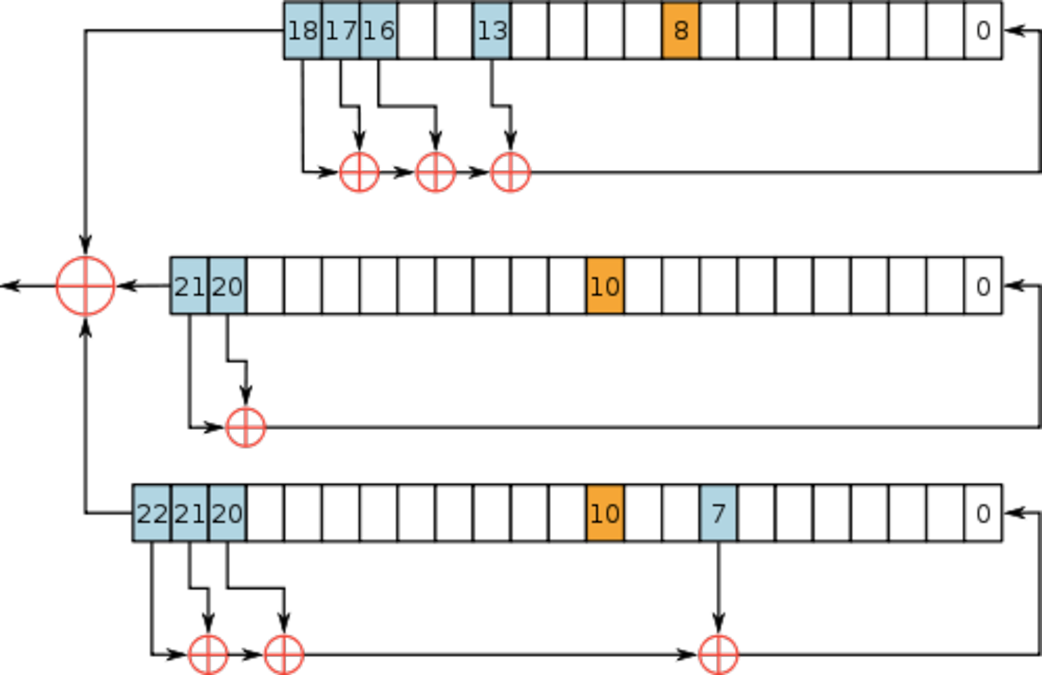
\includegraphics[width=50mm]{pic/A5-1_GSM_cipher} 
\end{center}
\end{figure}
\begin{alertblock}{WARNING}
Don't use any stream cipher. If necessary, construct one from a block cipher.
\end{alertblock}
\end{frame}
\begin{frame}\frametitle{Secure Multiple Encryptions Using a Stream Cipher}
\begin{figure}
\begin{center}
\begin{tikzpicture}
\node (sm) {};
\foreach \x in {1, 2, 3} {
\node (g\x) at ($(sm) + \x*(2.8cm,0) - (4cm,0)$)  [] {};
\node (pa\x) [right of = g\x, node distance = 1.8cm, minimum width = 2.8cm, draw] {Part \x};
\node (xor\x) [below of = pa\x, circle, node distance = 1cm, draw] {};
\draw[-] (xor\x.north) -- (xor\x.south);
\draw[-] (xor\x.east) -- (xor\x.west);
\node (pt\x) [left of = xor\x, node distance = 0.9cm] {$m_\x$};
\node (ct\x) [right of = xor\x, node distance = 0.8cm] {$c_\x$};
\draw[-latex] (pa\x) -- (xor\x);
\draw[-latex] (pt\x) -- (xor\x);
\draw[-latex] (xor\x) -- (ct\x);
}
\node (gg) at ($(sm) - (1.7cm,0)$)  [rounded corners=1ex,draw] {$G$};
\draw[-latex] (gg) -- (pa1);
\node (iv) [below=0.5cm of gg] {$K$};
\draw[-latex] (iv) -- (gg.south);
%\node (k) [left of = gg, node distance = 1cm] {$K$};
%\draw[-latex] (k) -- (gg);

\node (usm) [below of=sm, node distance=3.5cm] {};
\foreach \x in {1, 2, 3} {
\node (ug\x) at ($(usm) + \x*(3.3cm,0) - (5cm,0)$)  [rounded corners=1ex,draw] {$G$};
\node (uk\x) [above=0.5cm of ug\x] {};
\draw[-latex] (uk\x) -- (ug\x.north);
\node (uiv\x) [below=0.5cm of ug\x] {$IV_\x$};
\draw[-latex] (uiv\x) -- (ug\x.south);
\node (upa\x) [right of = ug\x, node distance = 1.8cm, minimum width = 2cm, draw] {Part \x};
\node (uxor\x) [below of = upa\x, circle, node distance = 1cm, draw] {};
\draw[-] (uxor\x.north) -- (uxor\x.south);
\draw[-] (uxor\x.east) -- (uxor\x.west);
\node (upt\x) [left of = uxor\x, node distance = 0.9cm] {$m_\x$};
\node (uct\x) [right of = uxor\x, node distance = 0.8cm] {$c_\x$};
\draw[-latex] (upa\x) -- (uxor\x);
\draw[-latex] (upt\x) -- (uxor\x);
\draw[-latex] (uxor\x) -- (uct\x);
\draw[-latex] (ug\x) -- (upa\x);
}
\draw[-] (uk1.south) node [left] {$K$} -- (uk3.south);
\node [above of= upt2, node distance=2.5cm] {\emph{Synchronized Mode}};
\node [below of= upt2] {\emph{Unsynchronized Mode}};
\end{tikzpicture}
\end{center}
\end{figure}
Initial vector $IV$ is chosen \emph{u.a.r} and public\\
\alert{Q: which mode is better in your opinion?}
\end{frame}
\begin{frame}\frametitle{Related Keys: Real World Cases}
Keys (the $IV$-key pair) for multiple enc. must be independent
\begin{exampleblock}{Attacks on 802.11b WEP}
Unsynchronized mode: $\mathsf{Enc}(m_i) := \left< IV_i, G(IV_i\|k) \oplus m_i\right>$\\
\begin{itemize}
\item Length of $IV$ is 24 bits, repeat $IV$ after $2^{24} \approx$ 16M frames
\item On some WiFi cards, $IV$ resets to $0$ after power cycle
\item $IV_i = IV_{i-1} + 1$. For RC4, recover $k$ after 40,000 frames
\end{itemize}
\end{exampleblock}
\end{frame}
\begin{frame}\frametitle{Chosen-Plaintext Attacks (CPA)}
\textbf{CPA}: the adversary has the ability to obtain the encryption of plaintexts of its choice
\begin{exampleblock}{A story in WWII}
\begin{itemize}
\item Navy cryptanalysts believe the ciphertext ``AF'' means ``Midway island'' in Japanese messages
\item But the general did not believe that Midway island would be attacked
\item Navy cryptanalysts sent a plaintext that the freshwater supplies at Midway island were low
\item Japanese intercepted the plaintext and sent a ciphertext that ``AF'' was low in water
\item The US forces dispatched three aircraft carriers and won
\end{itemize}
\end{exampleblock}
\end{frame}
\begin{frame}\frametitle{Security Against CPA}
The CPA indistinguishability experiment $\mathsf{PrivK}^{\mathsf{cpa}}_{\mathcal{A},\Pi}(n)$:
\begin{enumerate}
	\item $k \gets \mathsf{Gen}(1^n)$
	\item $\mathcal{A}$ is given input $1^n$ and \textbf{oracle access} $\mathcal{A}^{\mathsf{Enc}_k(\cdot)}$ to $\mathsf{Enc}_k(\cdot)$, outputs $m_0, m_1$ of the same length
	\item $b \gets \{0,1\}$. Then $c \gets \mathsf{Enc}_k(m_b)$ is given to $\mathcal{A}$
	\item $\mathcal{A}$ \textbf{continues to have oracle access} to $\mathsf{Enc}_k(\cdot)$, outputs $b'$
	\item If $b' = b$, $\mathcal{A}$ succeeded $\mathsf{PrivK}^{\mathsf{cpa}}_{\mathcal{A},\Pi}=1$, otherwise 0
\end{enumerate}
\begin{figure}
\begin{center}
\begin{tikzpicture}
\node (A) at (0,0) {\Homer};
\node (B) [right of = A, node distance = 4cm] {\Left\Burns};
\node (enc) [draw, rounded corners=1ex, right of=B, node distance = 2cm] {$\mathsf{Enc}_k(\cdot)$};
\draw[-latex] (B) to [bend left=15,-latex,above] (enc);
\draw[-latex] (enc) to [bend left=15,-latex,below] (B);
\node (k) [left of=A, node distance = 1.5cm] {Gen $k$};
\node (1a) [below of=A, node distance=1cm] {};
\node (1b) [below of=B, node distance=1cm] {$m_0, m_1$};
\draw[-latex] (1b) -- (1a) node [midway,above] {};
\node (2a) [below of=1a, node distance=0.5cm] {Gen $b$};
\node (2b) [below of=1b, node distance=0.5cm] {};
%\draw[-latex] (2b) -- (2a) node [midway,above] {};
%\node (3a) [below of=2a, node distance=0.5cm] {};
%\node (3b) [below of=2b, node distance=0.5cm] {};
\node (4a) [below of=2a, node distance=0.5cm] {$\mathsf{Enc}_k(m_b)$};
\node (4b) [below of=2b, node distance=0.5cm] {};
\draw[-latex] (4a) -- (4b) node [midway,above] {};
\node (5a) [below of=4a, node distance=0.5cm] {};
\node (5b) [below of=4b, node distance=0.5cm] {$b'$};
\draw[-latex] (5b) -- (5a) node [midway,above] {};
\node (6a) [below of=5a, node distance=0.5cm] {};
\node (6b) [below of=5b, node distance=0.5cm] {};
\node (result) [right of = 6a, node distance = 2cm] {Win if $b = b'$};
\end{tikzpicture}

\end{center}
\end{figure}
\end{frame}
\begin{frame}\frametitle{CPA Security for Multiple Encryptions}
\begin{definition}\label{def:cap-ind}
$\Pi$ has \textbf{indistinguishable encryptions under a CPA (CPA-secure)} if $\forall$ \textsc{ppt} $\mathcal{A}$, $\exists$ $\mathsf{negl}$ such that
\[ \Pr\left[\mathsf{PrivK}^{\mathsf{cpa}}_{\mathcal{A},\Pi}(n)=1\right] \le \frac{1}{2} + \mathsf{negl}(n).
\]
\end{definition}
\begin{itemize}
\item \alert{Q: Is any cipher we have learned so far CPA-secure? Why?}
\end{itemize}
\begin{proposition}
Any private-key encryption scheme that is CPA-secure also is \textbf{multiple-encryption} CPA-secure.
\end{proposition}
\begin{itemize}
\item \alert{Q: Does \textbf{multiple-encryption-security} mean CPA-security?} (homework)
%\item \textbf{Fixed-length} CPA-secure encryption scheme can be used to construct a \textbf{arbitrary-length} CPA-secure one quite easily.
\end{itemize}
\end{frame}
\section{Constructing CPA-Secure Encryption Schemes}
\begin{frame}\frametitle{Concepts on Pseudorandom Functions}
\begin{figure}
\begin{center}
\begin{tikzpicture}[uk/.style={inner sep=1pt, minimum width=10pt, circle, fill=red!50},kk/.style={inner sep=1pt, minimum width=10pt, fill=blue!50, circle}]
\node (K) at (2.2cm,0) [ellipse,minimum width=1cm,minimum height=2cm,draw] {}; 
\node (k) [above of=K,node distance=1.2cm] {$K$}; 
\foreach \i in {1, 2, 3} {
\node (X\i) at (\i*3.3cm,0) [ellipse,minimum width=1cm,minimum height=2cm,draw] {}; 
\node (x) [above of=X\i,node distance=1.2cm] {$X$}; 
\node (Y\i) [right of=X\i,ellipse,minimum width=1cm,minimum height=2cm,node distance=1.5cm,draw] {};
\node (y) [above of=Y\i,node distance=1.2cm] {$Y$}; 
}
\node (cr) at ($(X1)+(0cm,-1.5cm)$) [] {\footnotesize $F: K \times X \to Y$};
\node (cr) at ($(X1)+(0cm,-2cm)$) [] {\footnotesize 2D function};
\node (k1) at ($(K)+(0,0.3cm)$) [kk] {\tiny };
\node (k2) at ($(K)+(0,-0.3cm)$) [uk] {\tiny };
\node (x1) at ($(X1)+(0,0.3cm)$) [kk] {\tiny };
\node (x2) at ($(X1)+(0,-0.3cm)$) [kk] {\tiny };
\node (y1) at ($(Y1)+(0,0.3cm)$) [kk] {\tiny };
\node (y2) at ($(Y1)+(0,-0.3cm)$) [kk] {\tiny };
\draw[-latex,red!50] (x1) -- (y1);
\draw[-latex,red!50] (x2) -- (y2);
\draw[-latex] (x1) -- (y2);
\draw[-latex] (x2) -- (y1);
\draw[-] (k1) -- (x1);
\draw[-] (k1) -- (x2);
\draw[-,red!50] (k2) -- (x1);
\draw[-,red!50] (k2) -- (x2);
\node (2pr) at ($(X2)+(0.75cm,-1.5cm)$) [] {\footnotesize $F_k(x) \overset{\text{def}}{=} F(k,x)$};
\node (2pr) at ($(X2)+(0.75cm,-2cm)$) [] {\footnotesize Keyed function};
\node (x1) at ($(X2)+(0,0.3cm)$) [kk] {\tiny };
\node (x2) at ($(X2)+(0,-0.3cm)$) [kk] {\tiny };
\node (y1) at ($(Y2)+(0,0.3cm)$) [kk] {\tiny };
\node (y2) at ($(Y2)+(0,-0.3cm)$) [kk] {\tiny };
\draw[-latex] (x1) -- (y2);
\draw[-latex] (x2) -- (y1);
\node (pr) at ($(X3)+(0.75cm,-1.5cm)$) [] {\footnotesize $f : X \to Y$};
\node (pr) at ($(X3)+(0.75cm,-2cm)$) [] {\footnotesize Look-up table};
\node (x1) at ($(X3)+(0,0.3cm)$) [kk] {\tiny };
\node (x2) at ($(X3)+(0,-0.3cm)$) [kk] {\tiny };
\node (y1) at ($(Y3)+(0,0.3cm)$) [kk] {\tiny };
\node (y2) at ($(Y3)+(0,-0.3cm)$) [kk] {\tiny };
\draw[-latex] (x1) -- (y1);
\draw[-latex] (x2) -- (y1);
\end{tikzpicture}

\end{center}
\end{figure}
\begin{itemize}
\item \textbf{Keyed function} $F : \{0,1\}^* \times \{0,1\}^* \to \{0,1\}^*$ \\
$F_k : \{0,1\}^* \to \{0,1\}^*$, $F_k(x) \overset{\text{def}}{=} F(k,x)$
\item \textbf{Look-up table $f$}: $\{0,1\}^n \to \{0,1\}^n$ with size \alert{ = ? bits} %$n\cdot2^n$.
\item \textbf{Function family $\mathsf{Func}_n$}: all functions $\{0,1\}^n \to \{0,1\}^n$. $|\mathsf{Func}_n| = 2^{n\cdot2^n}$
\item \textbf{Length Preserving}: $\ell_{key}(n) = \ell_{in}(n) = \ell_{out}(n)$
\end{itemize}
\end{frame}
\begin{frame}\frametitle{Definition of Pseudorandom Function}
\textbf{Intuition}: A PRF $F$ generates a function $F_k$ that is indistinguishable from truly random selected function $f$ (look-up table) in $\mathsf{Func}_n$.\\ However, the function has \textbf{exponential length}. Give $D$ the deterministic \textbf{oracle access $D^{\mathcal{O}}$} to the functions $\mathcal{O}$.
\begin{definition}
An efficient length-preserving, keyed function $F$ is a \textbf{pseudorandom function (PRF)} if
$\forall\;$ \textsc{ppt} distinguishers $D$,
\[ \left|\Pr[D^{F_k(\cdot)}(1^n)=1] - \Pr[D^{f(\cdot)}(1^n)=1]\right| \le \mathsf{negl}(n),
\]
where $f$ is chosen \emph{u.a.r} from $\mathsf{Func}_n$.
\end{definition}
\begin{alertblock}{Q: Is the fixed-length OTP a PRF?}
\end{alertblock}
%\textbf{PRG vs. PRF}:
%\begin{itemize}
%\item Pseudorandomness over a set of strings vs. a set of functions.
%\item A PRG --- an instance of keyed PRF.
%\end{itemize}
%\textbf{Existence}: if PRG exists. In practice, block ciphers may be PRF.
\end{frame}
\begin{frame}\frametitle{Questions}
\begin{exampleblock}{Let $F: \{0,1\}^{n} \times \{0,1\}^{n} \to \{0,1\}^{n}$ be a secure PRF. Is $G$ a secure PRF?}
\begin{itemize}
\item $G((k_{1},k_{2}), x) = F(k_{1},x) \| F(k_{2},x)$
\item $G(k,x) = F(k, x\oplus 1^{n})$
\item $G(k,x) = reverse(F(k,x))$
\item $ G(k,x) = \left\{ 
  \begin{array}{l l}
    F(k,x) & \quad \text{when}\ x \neq 0^{n}\\
    0^{n} & \quad \text{otherwise}\\
  \end{array} \right. $
\item $ G(k,x) = \left\{ 
  \begin{array}{l l}
    F(k,x) & \quad \text{when}\ x \neq 0^{n}\\
    k & \quad \text{otherwise}\\
  \end{array} \right. $
\item $G(k,x) = F(k,x)\bigoplus F(k, x\oplus 1^{n})$
\end{itemize}
\end{exampleblock}
\end{frame}
\begin{frame}\frametitle{CPA-Security from Pseudorandom Function}
\begin{columns}[t]
\begin{column}{4cm}
\begin{figure}
\begin{center}
\begin{tikzpicture}
\node (r) {$r$};
\node (pg) [draw, below of = r, rounded corners=1ex,node distance = 1.5cm] {$F$};
\node (k) [left of = pg, node distance = 1.5cm] {$k$};
\node (pad) [minimum width=2cm, draw, shape = rectangle, below of = pg, node distance = 1.5cm] {Pad};
\node (xor) [below of = pad, circle, node distance = 1.2cm, draw] {};
\draw[-] (xor.north) -- (xor.south);
\draw[-] (xor.east) -- (xor.west);
\node (pt) [left of = xor, node distance = 1.5cm] {$m$};
\node (ct) [right of = xor, node distance = 1.5cm] {$c$};
\draw[-latex] (r) -- (pg);
\draw[-latex] (pg) -- (pad);
\draw[-latex] (pad) -- (xor);
\draw[-latex] (pt) -- (xor);
\draw[-latex] (xor) -- (ct);
\draw[-latex] (r) -| (ct);
\draw[-latex] (k) -- (pg);
\end{tikzpicture}
\end{center}
\end{figure}
\end{column}
\begin{column}{6cm}
\begin{construction}\label{thm:cpa}
\begin{itemize}
\item Fresh random string $r$.
\item $F_k(r)$: $\abs{k} = \abs{m} = \abs{r} = n$.
\item $\mathsf{Gen}$: $k \in \{0,1\}^n$.
\item $\mathsf{Enc}$: $s := F_k(r)\oplus m$, $c := \left<r, s\right>$.
\item $\mathsf{Dec}$: $m := F_k(r)\oplus s$.
\end{itemize}
\end{construction}
\begin{theorem}\label{thm:prf}
If $F$ is a PRF, this fixed-length encryption scheme $\Pi$ is CPA-secure.
\end{theorem}
\end{column}
\end{columns}
\end{frame}
\begin{frame}\frametitle{Proof of CPA-Security from PRF}
\textbf{Idea}: First, analyze the security in an idealized world where $f$ is used in $\tilde{\Pi}$; next, claim that if $\Pi$ is insecure when $F_k$ was used then this would imply $F_k$ is not PRF by reduction.
\begin{proof}
(1) Analyze $\Pr[\mathsf{Break}]$, $\mathsf{Break}$ means $\mathsf{PrivK}_{\mathcal{A},\tilde{\Pi}}^{\mathsf{cpa}}(n) = 1$:  \\
$\mathcal{A}$ collects $\{ \left< r_i, f(r_i) \right> \}$, $i=1,\dots,q(n)$ with $q(n)$ queries; \\
The challenge $c=\left<r_c, f(r_c)\oplus m_b\right>$. \\
\begin{itemize}
\item $\mathsf{Repeat}$: $r_c \in \{ r_i \}$ with probability $\frac{q(n)}{2^n}$. $\mathcal{A}$ can know $m_b$.
\item $\overline{\mathsf{Repeat}}$: As OTP, $\Pr[\mathsf{Break}]=\frac{1}{2}$ 
\end{itemize}
\[
\begin{split}
	\Pr[\mathsf{Break}] & =\Pr[\mathsf{Break} \land \mathsf{Repeat}] + \Pr[\mathsf{Break} \land \overline{\mathsf{Repeat}}] \\
	&\le \Pr[\mathsf{Repeat}] + \Pr[\mathsf{Break} | \overline{\mathsf{Repeat}}] \\
	&\le \frac{q(n)}{2^n} + \frac{1}{2}.
\end{split}
\]
\end{proof}
\end{frame}
\begin{frame}\frametitle{Proof of CPA-Security from PRF (Cont.)}
\begin{proof}
(2) Reduce $D$ to $\mathcal{A}$:
\begin{figure}
\begin{center}
\begin{tikzpicture}
\draw (0,0) rectangle (5,4);
\draw (4.25,0.2) rectangle (4.75,3);
\draw[-latex] (-2.5,3) -- (0,3) node [midway, above] {$\mathcal{O}: F_k$ or $f$} node [midway, below] {$1^n$};
\draw[-latex] (0,0.3) -- (-2.5,0.3) node [midway, above] {1 if $b' = b$};
\draw (1,3.5) node {{\Large $\mathcal{D}$}};
\draw (3,3.5) node {$b \gets \{0,1\}$};
\draw (4.5,1.75) node {\Large $\mathcal{A}$};
\draw[-latex] (4.25,2.5) -- (0.5,2.5) node [midway, above] {$m_0, m_1 \in \{0,1\}^{n}$};
\draw[-latex] (0.5,1.45) -- (4.25,1.45) node [midway, below] {$c:=\left<r, s' \oplus m_b\right>$} node [midway, above] {$s' = \mathcal{O}(r), r \gets \{0,1\}^{n}$};
\draw[-latex] (4.25,0.3) -- (0.5,0.3) node [midway, above] {$b'$};
\draw[-latex] (4.5,3.5) node[above] {$n$} -- (4.5,3);
\end{tikzpicture}
\end{center}
\end{figure}
{\footnotesize 
$ \Pr[D^{F_k(\cdot)}(1^n)=1] = \Pr[\mathsf{PrivK}_{\mathcal{A},\Pi}^{\mathsf{cpa}}(n) = 1] = \frac{1}{2} + \varepsilon(n). $
$ \Pr[D^{f(\cdot)}(1^n)=1] = \Pr[\mathsf{PrivK}_{\mathcal{A},\tilde{\Pi}}^{\mathsf{cpa}}(n) = 1] = \Pr[\mathsf{Break}] \le \frac{1}{2} + \frac{q(n)}{2^n}. $
$\Pr[D^{F_k(\cdot)}(1^n)=1] - \Pr[D^{f(\cdot)}(1^n)=1] \ge \varepsilon(n) - \frac{q(n)}{2^n}.$
$\varepsilon(n)$ is negligible.
}
\end{proof}
\end{frame}
\begin{frame}\frametitle{Remarks on CPA-Security from PRF}
\begin{itemize}
\item For arbitrary-length messages, $m = m_1, \dots , m_{\ell}$
\[ c := \left< r_1, F_k(r_1) \oplus m_1, r_2, F_k(r_2) \oplus m_2, \dots, r_\ell, F_k(r_\ell) \oplus m_\ell\right>
\]
\begin{corollary}
If $F$ is a PRF, then $\Pi$ is CPA-secure for arbitrary-length messages.
\end{corollary}
\item \textbf{Efficiency}: $|c| = 2|m|$. 
\end{itemize}
\end{frame}
\begin{frame}\frametitle{Pseudorandom Permutations}
\begin{itemize}
\item \textbf{Bijection}: $F$ is one-to-one and onto
\item \textbf{Permutation}: A bijective function from a set to itself
\item \textbf{Keyed permutation}: $\forall k, F_k(\cdot)$ is permutation
\item $F$ is a bijection $\iff F^{-1}$ is a bijection
\end{itemize}
\begin{definition}
An efficient, keyed permutation $F$ is a \textbf{strong pseudorandom permutation (PRP)} if
$\forall\;$ \textsc{ppt} distinguishers $D$,
\[ \left|\Pr[D^{F_k(\cdot),F_k^{-1}(\cdot)}(1^n)=1] - \Pr[D^{f(\cdot),f^{-1}(\cdot)}(1^n)=1]\right| \le \mathsf{negl}(n),
\]
where $f$ is chosen \emph{u.a.r} from the set of permutations on $n$-bit strings.
\end{definition}
\begin{alertblock}{If $F$ is a pseudorandom permutation then is it a PRF?}
\end{alertblock}
\end{frame}
\begin{frame}\frametitle{Questions}
\begin{exampleblock}{Let $X = \{ 0,1\}$ (1 bit), answer the following questions.}
\begin{enumerate}
\item What are the functions in the permutation over $X$?
\item $K = \{0, 1\}$, what is the simplest permutation $F(k, x)$ over $X$? 
\item Is your $F$ a secure PRP?
\item Is your $F$ a secure PRF?
\item What if $X = \{ 0,1\}^{128}$ and $K = \{0, 1\}^{128}$?
\item Could you give a (or another) PRP over $X = \{ 0,1\}^{128}$?
\end{enumerate}
\end{exampleblock}
\begin{proposition}
IF $F$ is a PRP and additionally $\ell_{in} (n) \ge n$, then $F$ is also a PRF.
\end{proposition}
\end{frame}
\section{Modes of Operation}
\begin{frame}\frametitle{PRF, PRP, PRG, and Modes of Operation}
\textbf{Modes of Operation:}
\begin{itemize} 
\item A way of encrypting arbitrary-length messages using a PRP or PRF
\item A way of constructing a PRG from a PRP or PRF
\end{itemize}
\end{frame}
\begin{frame}\frametitle{Electronic Code Book (ECB) Mode}
\begin{figure}
\begin{center}
\begin{tikzpicture}
\foreach \x in {1, 2, 3} {
\node (f\x) at ($\x*(2.5cm,0)$) [minimum size=1.25cm,rounded corners=1ex,draw] {\Large $F_k$};
\node (m\x) [above of=f\x, node distance=2cm] {$m_\x$};
\node (c\x) [below of=f\x, node distance=2cm] {$c_\x$};
\draw[-latex] (m\x) -- (f\x);
\draw[-latex] (f\x) -- (c\x);
}
\end{tikzpicture}

\end{center}
\end{figure}
\begin{itemize}
\item \alert{Q: is it indistinguishable in the presence of an eavesdropper?}
\item \alert{Q: can $F$ be any PRF?}
\end{itemize}
\end{frame}
\begin{frame}\frametitle{Attack on ECB mode}
\begin{figure}
\begin{center}
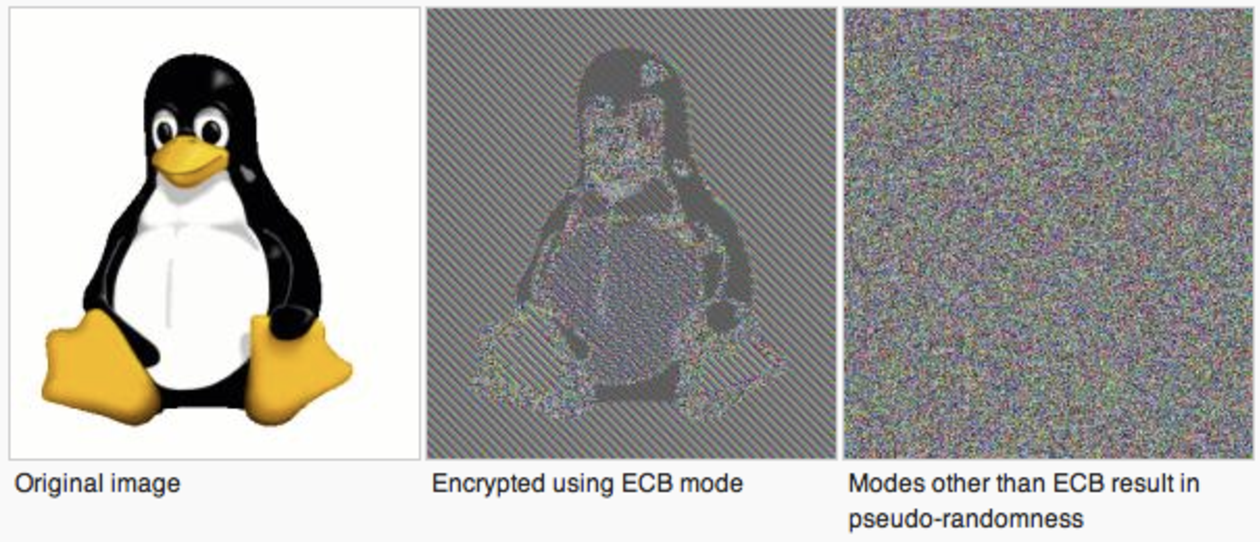
\includegraphics[width=100mm]{pic/ecb} 
\end{center}
\end{figure}
\end{frame}
\begin{frame}\frametitle{Cipher Block Chaining (CBC) Mode}
\begin{figure}
\begin{center}
\begin{tikzpicture}
\foreach \x in {1, 2, 3} {
\node (f\x) at ($\x*(2.5cm,0)$) [minimum size=1.25cm,rounded corners=1ex,draw] {\Large $F_k$};
\node (m\x) [above of=f\x, node distance=2.5cm] {$m_\x$};
\node (c\x) [below of=f\x, node distance=1.5cm] {$c_\x$};
\node (p\x) [above of=f\x, node distance=1.5cm, circle, draw] {};
\draw[-] (p\x.north) -- (p\x.south);
\draw[-] (p\x.east) -- (p\x.west);
\draw[-latex] (m\x) -- (p\x);
\draw[-latex] (p\x) -- (f\x);
\draw[-latex] (f\x) -- (c\x);
}

\node (iv) [left of=p1, node distance=1.5cm] {$IV$};
\node (iv2) [left of=c1, node distance=1.5cm] {$IV$};
\draw[-latex] (iv) -- (iv2);
\draw[-latex] (iv) -- (p1);

\foreach \x in {1, 2} {
\draw[-latex] ($(c\x) + (0,0.6cm)$) -| +(1.25cm,2.4cm) -- ($(p\x.west) + (2.5cm,0)$);
}

\end{tikzpicture}
\end{center}
\end{figure}
\begin{itemize}
\item $IV$: initial vector, a fresh random string.
\item \alert{Q: is it CPA-secure? what if $IV$ is always $0$?}
\item \alert{Q: is the encryption parallelizable, i.e., outputting $c_{2}$ before getting $c_{1}$?}
\item \alert{Q: can $F$ be any PRF?}
\end{itemize}
\end{frame}
\begin{frame}\frametitle{Output Feedback (OFB) Mode}
\begin{figure}
\begin{center}
\begin{tikzpicture}
\foreach \x in {1, 2, 3} {
\node (f\x) at ($\x*(2.5cm,0)$) [minimum size=1.25cm,rounded corners=1ex,draw] {\Large $F_k$};
\node (c\x) [below of=f\x, node distance=2.5cm] {$c_\x$};
\node (p\x) [below of=f\x, node distance=1.5cm, circle, draw] {};
\node (m\x) [left of=p\x, node distance=1.0cm] {$m_\x$};
\draw[-] (p\x.north) -- (p\x.south);
\draw[-] (p\x.east) -- (p\x.west);
\draw[-latex] (m\x) -- (p\x);
\draw[-latex] (f\x) -- (p\x);
\draw[-latex] (p\x) -- (c\x);
}

\node (iv2) [left of=c1, node distance=1.5cm] {$IV$};
\node (iv) [above of=iv2, node distance=4cm] {$IV$};
\draw[-latex] (iv) -- (iv2);
\draw[-latex] (iv) -| (f1.north);

\foreach \x in {1, 2} {
%\draw[-] ($(p\x) + (0,0.6cm)$) -| +(1.25cm,2.4cm);
%\draw[-latex] ($(p\x) + (1.25,3cm)$) -| ($(f\x.north) + (2.5cm,0)$);
\draw[-latex] ($(p\x) + (0,0.6cm)$) -| +(1.25cm,2.4cm) -| ($(f\x.north) + (2.5cm,0)$);
}

\end{tikzpicture}
\end{center}
\end{figure}
\begin{itemize}
\item \alert{Q: is it CPA-secure?}
\item \alert{Q: is the encryption parallelizable?}
\item \alert{Q: can $F$ be any PRF?}
\end{itemize}
\end{frame}
\begin{frame}\frametitle{Counter (CTR) Mode}
\begin{figure}
\begin{center}
\begin{tikzpicture}
\foreach \x in {1, 2, 3} {
\node (f\x) at ($\x*(2.5cm,0)$) [minimum size=1.25cm,rounded corners=1ex,draw] {\Large $F_k$};
\node (c\x) [below of=f\x, node distance=2.5cm] {$c_\x$};
\node (p\x) [below of=f\x, node distance=1.5cm, circle, draw] {};
\node (m\x) [left of=p\x, node distance=1.0cm] {$m_\x$};
\node (ctr\x) [above of=f\x, node distance=1.5cm] {$\mathsf{ctr}+\x$};
\draw[-] (p\x.north) -- (p\x.south);
\draw[-] (p\x.east) -- (p\x.west);
\draw[-latex] (m\x) -- (p\x);
\draw[-latex] (f\x) -- (p\x);
\draw[-latex] (p\x) -- (c\x);
\draw[-latex] (ctr\x) -- (f\x);
}
\node (iv2) [left of=c1, node distance=1.5cm] {$\mathsf{ctr}$};
\node (iv) [above of=iv2, node distance=4cm] {$\mathsf{ctr}$};
\draw[-latex] (iv) -- (iv2);
\end{tikzpicture}
\end{center}
\end{figure}
\begin{itemize}
\item $ctr$ is an $IV$
\item \alert{Q: is it CPA-secure?}
\item \alert{Q: is the encryption parallelizable?}
\item \alert{Q: can $F$ be any PRF?}\end{itemize}
\end{frame}
\begin{frame}\frametitle{CTR Mode Is CPA-secure}
\begin{theorem}
If $F$ is a PRF, then randomized CTR mode is CPA-secure.
\end{theorem}
\begin{proof}
The message length and the number of query are $q(n)$. \\
\textbf{Overlap}: the sequence for the challenge overlaps the sequences for the queries from the adversary.\\
$\mathsf{ctr}^*$: $\mathsf{ctr}$ in the challenge. $\mathsf{ctr}_i$: $\mathsf{ctr}$ in the queries, $i = 1,\dots,q(n)$.\\
$\mathsf{Overlap}$: $\mathsf{ctr}_i-q(n) < \mathsf{ctr}^* < \mathsf{ctr}_i + q(n)$.\\
\[\Pr[\mathsf{Overlap}] \le \frac{2q(n)-1}{2^n} \cdot q(n)\]
\end{proof}
\end{frame}
\begin{frame}\frametitle{Proof of CPA-secure CTR Mode (Cont.)}
\begin{proof}
See proof of theorem \ref{thm:prf}.
(1) Analyze $\mathsf{Break}$ : $\mathsf{PrivK}_{\mathcal{A},\tilde{\Pi}}^{\mathsf{cpa}}(n)=1$.
\[
\begin{split}
	\Pr[\mathsf{Break}] & =\Pr[\mathsf{Break} \land \mathsf{Overlap}] + \Pr[\mathsf{Break} \land \overline{\mathsf{Overlap}}] \\
	&\le \Pr[\mathsf{Overlap}] + \Pr[\mathsf{Break} | \overline{\mathsf{Overlap}}] \\
	&\le \frac{2q(n)^2}{2^n} + \frac{1}{2}.
\end{split}
\]
(2) Reduce $D$ to $\mathcal{A}$
\[ \Pr[D^{f(\cdot)}(1^n)=1]=\Pr[\mathsf{PrivK}_{\mathcal{A},\tilde{\Pi}}^{\mathsf{cpa}}(n)=1] \le \frac{2q(n)^2}{2^n} + \frac{1}{2}
\]
\[\Pr[D^{F_k(\cdot)}(1^n)=1]=\Pr[\mathsf{PrivK}_{\mathcal{A},\Pi}^{\mathsf{cpa}}(n)=1] \le \frac{1}{2} + \varepsilon(n)
\]
\[ \text{If } F \text{ is PRP}, \varepsilon(n) \text{ is negligible.}
\]
\end{proof}
\end{frame}
\begin{frame}[fragile]\frametitle{$IV$ Should Not Be Predictable}
If $IV$ is predictable, then CBC/OFB/CTR mode is not CPA-secure.\\
\alert{Q: Why? (homework)}
\begin{exampleblock}{Bug in SSL/TLS 1.0}
$IV$ for record $\#i$ is last CT block of record $\#(i-1)$.
\end{exampleblock}
\begin{exampleblock}{API in OpenSSL}
\verb#void AES_cbc_encrypt (# \\
\verb#    const unsigned char *in,# \\
\verb#    unsigned char       *out,# \\
\verb#    size_t              length,# \\
\verb#    const AES_KEY       *key,# \\
\verb#    unsigned char       *ivec,   #  \alert{\textbf{User supplies $IV$}} \\
\verb#    AES_ENCRYPT or AES_DECRYPT);# \\
\end{exampleblock}
\end{frame}
%\begin{frame}\frametitle{PRP/PRF Switching Lemma (FYI)}
%\begin{lemma}
%$\forall\;$ \textsc{ppt} distinguishers $D$,
%\[ \left|\Pr[D^{f}=1] - \Pr[D^{p}=1]\right| \le \frac{q^{2}}{2^{n+1}},
%\]
%where $f$/$p$ is chosen \emph{u.a.r} from the set of functions/permutations on $n$-bit strings.
%\end{lemma}
%\begin{exampleblock}
%\end{exampleblock}
%\end{frame}
\section{Security Against Chosen-Ciphertext Attacks (CCA)}
\begin{frame}\frametitle{Security Against CCA}
The CCA indistinguishability experiment $\mathsf{PrivK}^{\mathsf{cca}}_{\mathcal{A},\Pi}(n)$:
\begin{enumerate}
	\item $k \gets \mathsf{Gen}(1^n)$.
	\item $\mathcal{A}$ is given input $1^n$ and oracle access $\mathcal{A}^{\mathsf{Enc}_k(\cdot)}$ and $\mathcal{A}^{\mathsf{Dec}_k(\cdot)}$, outputs $m_0, m_1$ of the same length.
	\item $b \gets \{0,1\}$. $c \gets \mathsf{Enc}_k(m_b)$ is given to $\mathcal{A}$.
	\item $\mathcal{A}$ continues to have oracle access \alert{\textbf{except for $c$}}, outputs $b'$.
	\item If $b' = b$, $\mathcal{A}$ succeeded $\mathsf{PrivK}^{\mathsf{cca}}_{\mathcal{A},\Pi}=1$, otherwise 0.
\end{enumerate}
\begin{definition}
$\Pi$ has \textbf{indistinguishable encryptions under a CCA (CCA-secure)} if $\forall$ \textsc{ppt} $\mathcal{A}$, $\exists$ $\mathsf{negl}$ such that
\[ \Pr\left[\mathsf{PrivK}^{\mathsf{cca}}_{\mathcal{A},\Pi}(n)=1\right] \le \frac{1}{2} + \mathsf{negl}(n).
\]
\end{definition}
\end{frame}
\begin{frame}\frametitle{Understanding CCA-security}
\begin{itemize}
\item In real world, the adversary might conduct CCA by influencing what gets decrypted
\begin{itemize}
\item If the communication is not authenticated, then an adversary may send certain ciphertexts on behalf of the honest party
\end{itemize}
\item CCA-security implies ``\textbf{non-malleability}''
\item None of the above scheme is CCA-secure
\end{itemize}
\begin{exampleblock}{CCA against Construction \ref{thm:cpa}}
$\mathcal{A}$ gives $m_{0}, m_{1}$ and gets $c = \left<r, F_k(r)\oplus m_{b}\right>$, 
and then queries $c'$ which is the same with $c$ except that a single bit is flipped. 
The $m' = c' \oplus F_k(r)$ should be the same with $m_{b}$ \alert{except \underline{$\qquad$}?}
\end{exampleblock}
\alert{Q: Show that the above modes (CBC, OFB and CTR) are also not CCA-secure. (homework)}
\end{frame}
\begin{frame}\frametitle{Padding-Oracle Attacks}
\textbf{PKCK \#5 Padding}:  append $b$ bytes of $b$ to the message in order to make the total length a multiple of the block length (append a dummy block if needed). The decryption server will return a \textbf{Bad Padding Error} for incorrect padding.\\
\textbf{Padding-Oracle Attacks}: 
\begin{itemize}
\item In a one-block CBC, by modifying the 1st byte of $IV$, attacker can learn whether $m$ is NULL. If yes, error will occur. 
\end{itemize}
\begin{columns}[c]
\column{.5\textwidth}
\begin{figure}
\begin{center}
\begin{tikzpicture}[scale=0.7, every node/.style={scale=0.7}]
\foreach \x in {1, 2, 3} {
\node (f\x) at ($\x*(2.5cm,0)$) [minimum size=1.25cm,rounded corners=1ex,draw] {\Large $F_k$};
\node (m\x) [above of=f\x, node distance=2.5cm] {$m_\x$};
\node (c\x) [below of=f\x, node distance=1.5cm] {$c_\x$};
\node (p\x) [above of=f\x, node distance=1.5cm, circle, draw] {};
\draw[-] (p\x.north) -- (p\x.south);
\draw[-] (p\x.east) -- (p\x.west);
\draw[-latex] (m\x) -- (p\x);
\draw[-latex] (p\x) -- (f\x);
\draw[-latex] (f\x) -- (c\x);
}

\node (iv) [left of=p1, node distance=1.5cm] {$IV$};
\node (iv2) [left of=c1, node distance=1.5cm] {$IV$};
\draw[-latex] (iv) -- (iv2);
\draw[-latex] (iv) -- (p1);

\foreach \x in {1, 2} {
\draw[-latex] ($(c\x) + (0,0.6cm)$) -| +(1.25cm,2.4cm) -- ($(p\x.west) + (2.5cm,0)$);
}

\end{tikzpicture}
\end{center}
\end{figure}
\column{.5\textwidth}
\begin{itemize}
\item append $\{b\}^b$ as a dummy block if $m$ is NULL
\item change the 1st byte of $IV$ from $x$ to $y$, get decrypted block $(x \oplus y \oplus b) \| \{b\}^{b-1}$, and trigger an error
\end{itemize}
\end{columns}
\end{frame}
\begin{frame}\frametitle{Padding-Oracle Attacks (Cont.)}
\begin{figure}
\begin{center}
\begin{tikzpicture}[scale=0.7, every node/.style={scale=0.7}]
\foreach \x in {1, 2, 3} {
\node (f\x) at ($\x*(2.5cm,0)$) [minimum size=1.25cm,rounded corners=1ex,draw] {\Large $F_k$};
\node (m\x) [above of=f\x, node distance=2.5cm] {$m_\x$};
\node (c\x) [below of=f\x, node distance=1.5cm] {$c_\x$};
\node (p\x) [above of=f\x, node distance=1.5cm, circle, draw] {};
\draw[-] (p\x.north) -- (p\x.south);
\draw[-] (p\x.east) -- (p\x.west);
\draw[-latex] (m\x) -- (p\x);
\draw[-latex] (p\x) -- (f\x);
\draw[-latex] (f\x) -- (c\x);
}

\node (iv) [left of=p1, node distance=1.5cm] {$IV$};
\node (iv2) [left of=c1, node distance=1.5cm] {$IV$};
\draw[-latex] (iv) -- (iv2);
\draw[-latex] (iv) -- (p1);

\foreach \x in {1, 2} {
\draw[-latex] ($(c\x) + (0,0.6cm)$) -| +(1.25cm,2.4cm) -- ($(p\x.west) + (2.5cm,0)$);
}

\end{tikzpicture}
\end{center}
\end{figure}
\begin{itemize}
\item If no error, then learn whether $m$ is 1 byte by modifying the 2nd byte of $IV$ and so on (changing the ciphertext)
\item Once learn the length of $m$, learn the last byte of $m$ ($s$) by modifying the one before the last block in the ciphertext
\item $m_{last} = \cdots s \| \{b\}^{b}$, $c_{last-1} = \cdots t \| \{\cdot \}^{b} $
\item modify $c_{last-1}$ to $c_{last-1}' = \cdots u \| (\{\cdot \}^{b} \oplus \{b\}^{b} \oplus \{b+1\}^{b}) $
\item \alert{Q: If no padding error, then $s$ = ?}
% s ^ t = u  ^ (b+1),  s= u ^ (b+1) ^ t
\end{itemize}
\end{frame}
\begin{frame}\frametitle{Padding-Oracle Attacks: Real-world Case}
CAPTCHA server will return an error when deciphering the CT of a CAPTCHA text received from a user.
\begin{figure}
\begin{center}
\begin{tikzpicture}[font=\footnotesize]
\node (A) at (0,0) [label=below:User] {\Lisa};
\node (B) [right of = A, node distance = 4cm,label=below:Web Server] {\Left\Bart};
\node (C) at (2,4) [rounded corners=1ex,minimum width=2cm,label distance=-2cm] {\Homer};
\node at (3.5,3.5) {CAPTCHA Server};  
\draw[-latex] (B) -- (A) node [midway,above] {(1) $Enc_k(w)$};
\draw[-latex] (A.350) -- (B.190) node [midway,below] {(4) $w$};
\draw[-latex] (A.90) -- (C.240) node [sloped,midway,above] {(2) $Enc_k(w)$};
\draw[-latex] (C.250) -- (A.80)  node [sloped,midway,below] {(3) Image of $w$ or error};
\draw[latex-latex] (C.320) -- (B.70) node [sloped,midway,above] {(0) shared key $k$};
\end{tikzpicture}
\end{center}
\end{figure}
\end{frame}
\begin{frame}\frametitle{Summary}
\begin{itemize}
\item Asymptotic approach, proof of reduction, indistinguishable
\item PRG, PRF, PRP, stream cipher, block cipher
\item Security/construction against eavesdropping/CPA
\item EBC, CBC, OFB, CTR
\item CCA, padding-oracle attack
\end{itemize}
\end{frame}
\end{document}
